%
% File ucca_parsing.tex
%

\documentclass[11pt]{article}
\usepackage{acl2016}
\usepackage{times}
\usepackage{url}
\usepackage{latexsym}
\usepackage{pgfplotstable}
\usepackage[]{algorithm2e}
\usepackage{hyperref}
\usepackage{color}
\usepackage{lipsum,adjustbox}
\usepackage{tikz}
\usepackage{tikz-dependency}
\usetikzlibrary{shapes,fit,calc,er,positioning,intersections,decorations.shapes,mindmap,trees}
\tikzset{decorate sep/.style 2 args={decorate,decoration={shape backgrounds,shape=circle,shape size=#1,sha
pe sep=#2}}}

\newcommand{\oa}[1]{\footnote{\color{red} #1}}
\newcommand{\daniel}[1]{\footnote{\color{blue} #1}}
\newcommand{\com}[1]{}
\newcommand{\secref}[1]{Section \ref{#1}}

%\aclfinalcopy % Uncomment this line for the final submission
%\def\aclpaperid{***} %  Enter the acl Paper ID here

% To expand the titlebox for more authors, uncomment
% below and set accordingly.
% \addtolength\titlebox{.5in}    

\newcommand\BibTeX{B{\sc ib}\TeX}


\title{Broad-Coverage Semantic Constituency Parsing: \\
A Transition-Based Approach}
  %General Transition-Based Broad-Coverage Semantic Parsing

\author{Daniel Hershcovich \and Omri Abend \and Ari Rappoport \\
  Institute of Computer Science \\
  Hebrew University of Jerusalem \\
  {\tt \{danielh,oabend,arir\}@cs.huji.ac.il}
}

\date{}


\begin{document}
\maketitle

%%%%%%%%%%%%%%%%%%%%%%%%%%%%%%%%%%%%%%%%%%%%%%%%%%%%%%%%%%%%%%%
%%%%%%%%%%%%%%%%%     Abstract
%%%%%%%%%%%%%%%%%%%%%%%%%%%%%%%%%%%%%%%%%%%%%%%%%%%%%%%%%%%%%%%
\begin{abstract}

  Representing many common semantic phenomena requires more expressive formalisms
  than the ones commonly used for syntactic parsing. For instance, arguments that are shared
  between predicates are often semantically represented as multi-parented nodes,
  yielding DAG, rather than tree, structures.
  %which has lead to renewed interest in DAG parsing in recent years.
  Recent work has focused on broad-coverage semantic parsing into dependency
  (i.e., word-to-word) or abstract (i.e., not grounded in the words and phrases of the sentence) representations.
  We advocate a constituency-based formulation of the task and
  define the broad-coverage constituency semantic parsing task (henceforth, {\it BCSP}),
  and explore two approaches to tackle it, using the English UCCA corpus for our experiments.
  In one, we covert the UCCA structures into two related formalisms, and use existing
  state-of-the-art parsers for these settings.
  In the other, we construct a novel parser for the task.
  %  building on recent advances in discontiguous constituency parsing.
  Motivated by their high performance and conceptual simplicity,
  our exploration focuses on transition-based parsing.
  %We experiment with two types of semantic representations, obtaining encouraging results.
  
  %Universal Conceptual Cognitive Annotation (UCCA) is a semantic grammatical scheme
  % that assigns 
  %a complete structure to natural language text. We present the first automatic
  % UCCA parser, 
  % a transition-based parser using a novel transition system. We compare the
  % results to baselines 
  % obtained by converting UCCA to CoNNL-X, and training syntactic parsers on the
  % converted dependency trees.
  
\end{abstract}



%%%%%%%%%%%%%%%%%%%%%%%%%%%%%%%%%%%%%%%%%%%%%%%%%%%%%%%%%%%%%%%
\section{Introduction}

% (1) there has been much interest lately in broad-coverage semantic parsing.
%  (2) semantic parsing requires the development of new parsing technology
% (beyond syntactic parsers), as they are formally different. importantly, they
%  are not trees, but DAGs (e.g., argument sharing in control structures;
% see Oepen et al., 2015, AMR).

The formal constraints imposed by available statistical parsers are insufficient for
broad-coverage semantic parsing \cite{oepen2015semeval}.
Commonly imposed constraints, such as that the parse is a tree, are arguably reasonable for
accounting for the syntax of natural language, but are lacking when applied to semantic parsing,
as they are unable to capture argument sharing phenomena, such as control or coordination.
Indeed, all broad-coverage semantic schemes used in NLP we are aware of allow multiple parents.

Most work on broad-coverage semantic parsing has focused on semantic role labeling,
which is limited by its focus on shallow predicate-argument structures and predominantly on verbal
predicates. Abstract Meaning Representation (AMR) \cite{banarescu2013abstract},
which has attracted considerable attention recently,
provides a more complete semantic annotation in the form of elaborate graphs,
which account for a wider range of predicates, linkage and coreference phenomena.
Formally, it represents sentences as directed graphs, without grounding its
semantic sub-parts in the sentence's words and constituents.
Another line of work that addresses parsing into elaborate semantic structures,
is that of Broad-coverage Semantic Dependency Parsing \cite{oepen2014semeval,oepen2015semeval} (SDP).
Like AMR, SDP also addresses a wide range of argument structures (including verbal, nominal and adjectival ones)
and the inter-relations between them, but uses word-to-word dependency structures.
SDP has been explored in two recent SemEval tasks, exploring three approaches
for semantic representation: the Prague
Dependency Treebank tectogrammatical layer \cite{bohmova2003prague},
HSPG-derived parsers using the Enju parser\footnote{See \url{http://kmcs.nii.ac.jp/enju/}.},
and dependencies derived from the Lingo ERG
Minimal Recursion Semantics represenations \cite{Flic:02}.

Purely bi-lexical dependency representation necessarily requires arbitrary decisions regarding the representation (1) of constructions that have more than a single
head (e.g., coordination), (2) of cases where the identity of the head is disputed
(e.g., determiner-noun, preposition-noun etc.), and (3) of multi-word expressions,
which are semantically opaque and hence have no clear head. Under dependency representation
the treatment of these constructions is often unsystematic, yielding both conceptual
and practical problems \cite{schwartz2011neutralizing,Ivanova2012who,tsarfaty2012cross}.
In this work, we propose the task of broad-coverage semantic {\it constituency} parsing. 
Constituency representation of semantics has considerable advantage over dependency representation, as it does not force the idea of a single head: the units in a construction may simply be annotated as the children of a common non-terminal parent.

A general parser for this setting must support the prediction of multiple parents,
as well as of discontiguous constituents, both pervasive phenomena in semantic
structures even in English. Multiple parents show up frequently in the context of argument
sharing, where a certain argument participates in several relations but is only mentioned once.
Common examples are coordination structures
(e.g., in ``John went home and took a shower'', ``John'' is an argument of both ``went'' and ``took'')
or nominalizations (e.g., ``After graduation, John moved to London'', where ``John'' is an argument
of both ``graduation'' and ``moved'').
Discontiguous units are common even in syntactic structures in some languages (e.g., German, Bulgarian,
Korean and many others \cite{kallmeyer2013data}), and can even be found in English, e.g., in reported
speech: ``'The dog', John said, 'is back again''', and are even more pervasive in English semantic parses
(see \secref{sec:data}).

The only corpora we are aware of that annotates text with constituency semantic annotation are
corpora annotated according to the UCCA scheme \cite{abend2013universal,sulem2015conceptual}.
In order to assess the ability of existing technology to tackle the task,
we create converters between the UCCA annotation and CoNLL-style dependencies, as well as
discontiguous constituency trees, apply state-of-the-art parsers to these formalisms on
the converted representations, and convert them back into UCCA annotations.
We take a transition-based approach, motivated by the effectiveness of the approach in
related parsing tasks, as well as its computational efficiency and its conceptual simplicity.
Finally, we present a novel transition-based constituency parser that supports both discontiguous
constituents and multiple parents. To our knowledge, this is the first parser to tackle the task.
We apply the parser both to an in-domain and out-of-domain scenario.
Our experimental results shed light on the difficulty of the task, as well as the ability of
transition-based parsers to tackle it.

The contribution of this work is thus three-fold. First, we motivate and tackle the constituency broad-coverage
semantic parsing task. Second, we create converters, and assess the ability of existing parsing technology
for formally related settings to address the task, focusing on transition-based methods.
Third, we present the first parser for the task, as well as a first parser for UCCA.
All converters, parsers and datasets will be made publicly available upon publication.

\begin {figure*}
\begin{adjustbox}{width=\textwidth}
  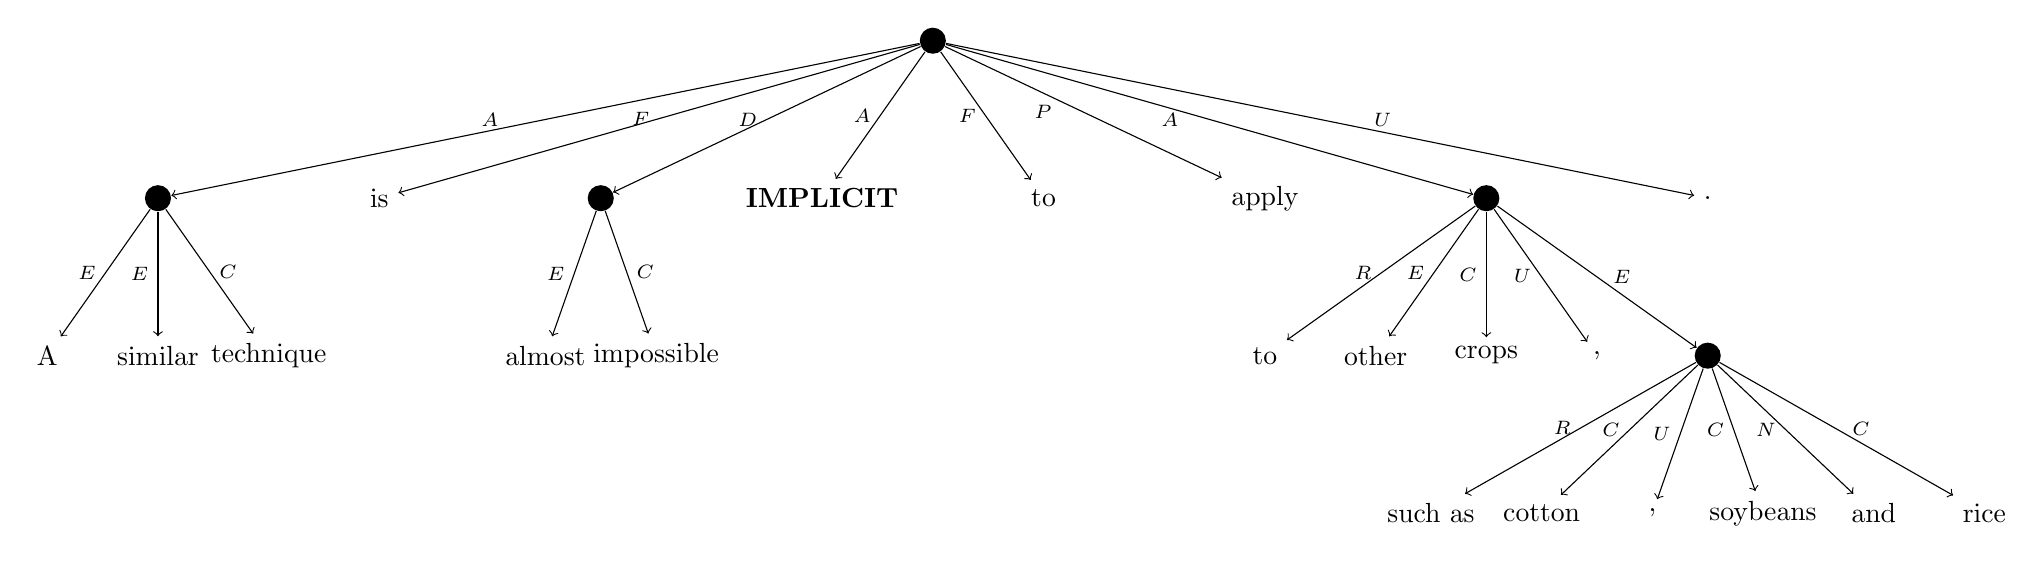
\begin{tikzpicture}[level distance=20mm, ->,
  level 1/.style={sibling distance=8em},
  level 2/.style={sibling distance=4em},
  level 3/.style={sibling distance=4em}]
    \label{fig:similar_technique}
    \node (ROOT) [fill=black, circle] {}
      child {node [fill=black, circle] {}
      {
        child {node {A} edge from parent node[left] {\scriptsize $E$}}
        child {node {similar} edge from parent node[left] {\scriptsize $E$}}
        child {node {technique} edge from parent node[right] {\scriptsize $C$}}
      } edge from parent node[left] {\scriptsize $A\quad$ \hspace{1mm} } }
      child {node {is} edge from parent node[left] {\scriptsize $F$}}
      child {node [fill=black, circle] {}
      {
        child {node {almost} edge from parent node[left] {\scriptsize $E$}}
        child {node {impossible} edge from parent node[right] {\scriptsize $C$}}
      } edge from parent node[left] {\scriptsize $D$} }
      child {node {\textbf{IMPLICIT}} edge from parent node[left] {\scriptsize $A$}}
      child {node {to} edge from parent node[left] {\scriptsize $F$}}
      child {node {apply} edge from parent node[left] {\scriptsize $P\quad$}}
      child {node [fill=black, circle] {}
      {
        child {node {to} edge from parent node[left] {\scriptsize $R$}}
        child {node {other} edge from parent node[left] {\scriptsize $E$}}
        child {node {crops} edge from parent node[left] {\scriptsize $C$}}
        child {node {,} edge from parent node[left] {\scriptsize $U$}}
        child {node [fill=black, circle] {}
        {
          child {node {such as} edge from parent node[left] {\scriptsize $R$}}
          child {node {cotton} edge from parent node[left] {\scriptsize $C$}}
          child {node {,} edge from parent node[left] {\scriptsize $U$}}
          child {node {soybeans} edge from parent node[left] {\scriptsize $C$}}
          child {node {and} edge from parent node[left] {\scriptsize $N$}}
          child {node {rice} edge from parent node[right] {\scriptsize $\; C$}}
        } edge from parent node[right] {\scriptsize $\; E$ \hspace{1mm} } }
      } edge from parent node[left] {\scriptsize $A\;$ \hspace{1mm} } }
      child {node {.} edge from parent node[right] {\scriptsize $\quad \quad U$}}
      ;
  \end{tikzpicture}
\end{adjustbox}
\end{figure*}

%%%%%%%%%%%%%%%%%%%%%%%%%%%%%%%%%%%%%%%%%%%%%%%%%%%%%%%%%%%%%%%
\section{Related work}

While no previous work has tackled the task of broad-coverage semantic constituency, 
the task resembles other statistical and semantic parsing tasks. The techniques used
in this work are closely related to some of them.

\paragraph{Semantic Parsing.}

% Brief, but broad. SRL, AMR, broad-coverage dependency, Boxer (and Groningen Meaning Bank), CCG-based.
% mention various graph parsing methods here
UCCA is similar to AMR~\cite{flanigan2014discriminative,artzi2015broad}.

\paragraph{Transition-based Parsing.}

\paragraph{Parsing with discontiguous untis.}
% cover both constituency and dependency-based approaches
\oa{Who to compare to? (we take a transition-based approach; later we discuss,
  without comparing, to grammar-based
  or graph-based approaches)
  Constituency parsers that meet some of the critera: Wolfgang's (all but multiple parents),
        which is state-of-the-art on Negra discontiguous units.
        There are no multiple parent constituency parsers! (so we can't compare)
  Dependency parsers: there are the standard ones (done!), there is MALT non-projective, and there is not MALT with mutliple parents. There are other dependency with multiple parents: tokgoez and erdigit (based on earlier work by sagae and tsujii) -- we're trying to get their code.
  
  We'll also say that future work will address other languages, ...
  Evaluation specifically on multiple parents, and on discontiguous.
  Future work: LSTM-version of our parser, conversion from t-layer parsers and such.
}

Syntactic dependency trees can in general be non-projective. Graph-based parsers are able to produce such trees, but many transition-based parsers assume projectivity to improve the performance and efficiency of the parser: the number of transitions in such parsers is always $2n$ where $n$ is the number of tokens \cite{nivre2004incrementality}. However, non-projective dependency trees can also be parsed by transition-based parsers in empirical linear time \cite{nivre2009non}.

In a UCCA graph, labels appear on the edges, whereas nodes are unlabeled. If all the nodes are known, parsing is the same as inducing a graph on them with the correct edge labels. In dependency parsing, a graph is induced on the set of nodes consisting of the tokens in the sentence (and the \textsc{ROOT} symbol). Therefore, it seems that techniques from dependency parsing can be used for UCCA parsing as well.

\paragraph{Other Semantic Schemes.}

Although the labels in a UCCA graph are on the edges, it is similar to phrase structure grammar: non-terminal units are internal nodes in the graph, rather than all the edges being between words in the original sentence. In a constituency tree, constituents form a hierarchy above the words of the sentence.

Methods for constituent parsing can also be useful for UCCA parsing, but the common chart-based approach is also $\mathcal{O}(n^3)$ at best. However, there are also transition-based constituent parsers~\cite{zhu2013fast} with linear run-time complexity.

Like standard dependency parsers, transition-based constituent parsers are generally unable to produce \textit{discontinuous constituents} (the equivalent of non-projective dependency trees). However, Maier~\shortcite{maier2015discontinuous} introduced a transition-based constituent parsing with a \textsc{swap} transition to allow discontinuous parsing.\footnote{https://github.com/wmaier/uparse}


%%%%%%%%%%%%%%%%%%%%%%%%%%%%%%%%%%%%%%%%%%%%%%%%%%%%%%%%%%%%%%%
\section{Conversion-based Approaches}

To our knowledge, there is no existing model to learn the general structure of UCCA graphs. Instead, as a baseline, we use models originally designed for syntactic dependency parsing, and train them on converted UCCA graphs. Since the converted annotation is not as rich as the UCCA scheme, some information is lost and has to be recovered as part of the conversion, so the accuracy of this method is bounded by the conversion accuracy.

\subsection{Conversion to dependency tree}

Since existing dependency parsers rely on specific annotation formats that are different from the UCCA graph annotation, we had to perform a conversion. We chose the CoNLL-X format, which is common among dependency parsers.
The top two rows in Table~\ref{table:convert} show the accuracy of conversion from UCCA to CoNLL-X and then back to UCCA.

\subsubsection{Conversion from UCCA to CoNLL-X}

The conversion relies on several concepts: since UCCA has non-terminal units, whereas in CoNLL-X all edges are between tokens, each non-terminal unit $u$ in UCCA requires a representative terminal unit $t$ to be selected for it. $t$ is referred to as the \textit{head terminal} of $u$, and denoted $head(u)$. The edges on the path from $u$ to $t$ are referred to as \textit{head edges}, and the dependent of a head edge is a \textit{head child}. The head terminal of a unit is selected by selecting a head child iteratively. The head child tag of $u$ is the first among a pre-determined list of tags of which $u$ has outgoing edges, and the head child is any child of that type. The order of tags is: \textsc{C,N,H,P,S,A,D,T,E,R,F,L,LR,LA,G,Terminal} and \textsc{U}.

Since UCCA forms a DAG and not necessarily a tree, $t$ can be the head terminal of more than one unit. A \textit{top headed unit} of $t$ is any non-terminal unit $u$ such that $t$ is a head terminal of $u$, but not of any of $u$'s parents (if there are any). Denote by $top(t)$ an arbitrarily selected top headed unit of $t$.

The conversion is shown in Algorithm~\ref{alg:ucca2conll}.
\daniel{Is it really important to show the algorithm? If so, I need to correct it a little bit. Also, why didn't I use McDonald et al.'s conversion with custom head rules? There is also a long description of the conversion process in \url{http://hall.maltparser.org/cv/pub/johan_hall_phdthesis.pdf}}

\begin{algorithm}
 \KwData{UCCA graph $G$}
 \KwResult{CoNLL-X dependency tree $T$}
 $V(T) \leftarrow \emptyset$\\
 $E(T) \leftarrow \emptyset$\\
 \ForEach{$t \in \mathrm{terminals}(G)$}{
  $u \leftarrow top(t)$\\
  $p \leftarrow parent(u)$\\
  $t^\prime \leftarrow head(p)$\\
  $\ell \leftarrow \ell_G(p, u)$\\
  $V(T) \leftarrow V(T) \cup \{t\}$\\
  $E(T) \leftarrow E(T) \cup \{(t^\prime, t, \ell)\}$\\
 }
 \caption{UCCA to CoNLL-X Conversion}
 \label{alg:ucca2conll}
\end{algorithm}

\subsubsection{Conversion from CoNLL-X to UCCA}

A UCCA graph is created from a CoNLL-X dependency annotation using the following procedure: first, the dependency nodes (the tokens) are sorted topologically.

When a new edge is added, its tag is either the relation associated with the corresponding dependency arc, or, if no such arc exists, determined heuristically:
\begin{itemize}
\item If the child is a punctuation terminal, the tag is $U$;
\item otherwise, if the parent has a child with an $H$ tag, the tag is also $H$;
\item otherwise, if the parent has a child with an $A$ tag, the tag is $P$;
\item otherwise, the tag is $C$.
\end{itemize}

Algorithm~\ref{alg:conll2ucca} shows the conversion.

\begin{algorithm}
 \KwData{CoNLL-X dependency tree $T$}
 \KwResult{UCCA graph $G$}
 $r \leftarrow Node()$\\
 $V(G) \leftarrow r$\\
 $E(G) \leftarrow \emptyset$\\
 \ForEach{$t \in V(T)$}{
  $u \leftarrow Node()$\\
  $V(G) \leftarrow V(G) \cup \{t, u\}$\\
  $E(G) \leftarrow E(G) \cup \{(u, \textsc{Terminal}, t\}$\\
  \eIf{$\ell_T(t) = \textsc{Root}$}{
   $E(G) \leftarrow E(G) \cup \{(r, label(u), u\}$\\
  }{
   $p \leftarrow preterminal(parent(t))$\\
   $E(G) \leftarrow E(G) \cup \{(p, label(u), u\}$\\
  }
 }
 \caption{CoNLL-X to UCCA Conversion}
 \label{alg:conll2ucca}
\end{algorithm}

\subsection{Parsing using dependency parsers}

In order to provide a baseline for UCCA parsing, we trained two state-of-the-art dependency parsers on a dataset resulting from conversion of the UCCA corpus to CoNLL-X format. Then we ran the resulting parser models, converted the results to the UCCA format, and evaluated using the labeled F1, unlabeled F1 and weakly labeled F1 measures. The results are shown in Table~\ref{table:convert}.

%\subsection{Conversion to dependency DAG}
%
%TODO: convert to (projective) dependency DAG
%
%\subsection{Parsing using DAG parsers}
%
%TODO: use Tokg\"oz and Eryi\u{g}it's parser to parse converted DAGs \cite{tokgoz2015transition}

\subsection{Conversion to constituency tree}

Another common format is constituency trees. Here, the conversion is relatively simple: we just remove remote and linkage edges, and all linkage and implicit nodes. This results in a tree that can be parsed by constituency parsers.

\subsection{Parsing using constituency parsers}

The conversion results in constituency trees, but some of the nodes may have a discontinuous yield. Most transition-based parsers are unable to deal with such trees, but we used \textsc{uparse} \cite{maier2015discontinuous}, which is able to parser discontinuous structures. The results are shown in Table~\ref{table:convert}.

%%%%%%%%%%%%%%%%%%%%%%%%%%%%%%%%%%%%%%%%%%%%%%%%%%%%%%%%%%%%%%%
\section{Direct Approach}

\subsection{Task definition}

Assuming a pre-defined set $L$ of edge tags, a \textit{UCCA graph} for a text $x=w_1 \ldots w_n$ is a directed graph $G=(V,E)$, where:
\begin{enumerate}
 \item $V$ is a set of nodes s.t. $\{w_1, \ldots, w_n\} \subseteq V$,
 \item $E \subseteq V \times L \times V$ is a set of labeled edges.
\end{enumerate}
The set $V$ of nodes consists of the \textit{terminal} nodes $w_1, \ldots, w_n$, and the non-terminal nodes. The set $E$ of edges is a set of triplets $(u, \ell, v)$, where $u$ and $v$ are nodes and $\ell$ is an edge tag.

In UCCA parsing, $x$ is given and the task is to build $G$.

\subsection{Transition-based UCCA parser}

Many approaches could be used to create a parser for UCCA, such as the graph-based approach
employed in JAMR~\cite{flanigan2014discriminative}.
We chose to adopt the transition-based approach for parsing UCCA.

We define a transition system for UCCA parsing as a quadruple $S=(C,T,c_s,C_t)$, where
\begin{enumerate}
 \item $C$ is a set of configurations.
\end{enumerate}

Our parser architecture combines transition-based constituency parsers \cite{zhu2013fast,maier2015discontinuous} with transition-based DAG dependency parsers \cite{sagae2008shift,tokgoz2015transition}:

\begin{itemize}
	\item Parsing starts with the root node on the stack.
	\item \textsc{Node$_X$} creates a new node on the buffer head as a parent of the first element on the stack (with edge tag $X$), but it does not reduce the first element on the stack; since nodes in UCCA may have multiple parents, they should only be reduced after all their edges have been created.
	\item \textsc{Left-Edge$_X$} and \textsc{Right-Edge$_X$} create a new edge between the first two elements on the stack, but again, they do not reduce any of them, to allow for multiple parents.
	\item \textsc{Left-Remote$_X$} and \textsc{Right-Remote$_X$} are identical to \textsc{Left-Edge$_X$} and \textsc{Right-Edge$_X$}, except that the edges they create are marked as remote. In UCCA there may be long-distance edges, called remote edges.
	\item \textsc{Implicit$_X$} is identical to \textsc{Node$_X$} action, except that the node created by it becomes the child of the stack top rather than its parent, and is marked implicit. Some non-terminal units are implicit units, meaning they do not correspond to any terminals. We add the constraint that implicit nodes cannot have any children.
\end{itemize}

The transitions are:

\textsc{Node$_X$, Implicit$_X$, Left-Edge$_X$, Right-Edge$_X$, Left-Remote$_X$, Right-Remote$_X$, Reduce, Shift, Swap, Finish}

\subsection{Constraints}
Each action has a set of constraint that must be met for that action to be possible. If any of the constraint is not met, the parser may not take that action. The constraints are:
\begin{description}
	\item[\textsc{Finish}] the root node has at least one child.
	\item[\textsc{Shift}] buffer is not empty.
	\item[\textsc{Node$_X$}] stack is not empty, $s_0$ is not the root node, and $X$ is T iff $s_0$ is a terminal.
	\item[\textsc{Implicit$_X$}] stack is not empty, and $s_0$ is not a terminal and not an implicit node.
	\item[\textsc{Reduce$_X$}] stack is not empty, and if $s_0$ is the root node, it has at least one child.
	\item[\textsc{Left-Edge$_X$}] stack has at least two elements, $s_0$ is not a terminal, $s_1$ is not the root node, $s_0$ is not the root node if $s_1$ is a terminal, the edge does not already exist, and $X$ is T iff $s_1$ is a terminal.
	\item[\textsc{Right-Edge$_X$}] stack has at least two elements, $s_1$ is not a terminal, $s_0$ is not the root node, $s_1$ is not the root node if $s_0$ is a terminal, the edge does not already exist, and $X$ is T iff $s_0$ is a terminal.
	\item[\textsc{Left-Remote$_X$}] stack has at least two elements, $s_0$ is not a terminal, $s_1$ is not the root node, $s_0$ is not the root node if $s_1$ is a terminal, the edge does not already exist, $X$ is T iff $s_1$ is a terminal, $s_0$ has at least one child, and $s_1$ has at least one parent.
	\item[\textsc{Right-Remote$_X$}] stack has at least two elements, $s_1$ is not a terminal, $s_0$ is not the root node, $s_1$ is not the root node if $s_0$ is a terminal, the edge does not already exist, $X$ is T iff $s_0$ is a terminal, $s_1$ has at least one child, and $s_0$ has at least one parent.
	\item[\textsc{Swap}] stack has at least two elements, .
\end{description}

\subsection{Feature representation}
\label{subsec:features}

Fig.~\ref{fig:features} shows the features templates adapted from Maier~\shortcite{maier2015discontinuous}. $s_i$ and $b_i$ stand for the $i$th stack and buffer items respectively, $w$ stands for the head word (see~\ref{subsec:head_rules}), $t$ for its POS tag, $e$ for the head incoming edge label. Note that $e$ replaces $c$ (consituent label) from Maier~\shortcite{maier2015discontinuous}, since in UCCA the labels are on the edges rather than the units; and a unit may have more than one incoming edge. $l$ and $r$ ($ll$ and $rr$) represent the leftmost and rightmost children (grand-children) of the element; $u$ handles the unary case.
Concerning the separator features, $p$ is a unique separator feature between the head words of $s_0$ and $s_1$; $q$ is the count of any separator features between them.
$x$ denotes the gap type of a subgraph. There are three possible values, either "none" (fully continuous), "pass" (there is a gap at the root, i.e., this gap must be filled later further up in the graph), or "gap" (the root of this graph fills a gap, i.e., its children have gaps, but the root does not). Finally, $y$ is the sum of all gap lengths.

Fig.~\ref{fig:new_features} shows the features templates introduced in this work. $P$ stands for the number of parents a node currently has, and $C$ for the number of children.

% FEATURES
\begin{figure}[t]
\begin{description}
	\item[unigrams] \hfill \\
	$s_0te, s_0we, s_1te, s_1we, s_2te, s_2we, s_3te, s_3we,$ \\
	$b_0wt, b_1wt, b_2wt, b_3wt,$ \\
	$s_0lwe, s_0rwe, s_0uwe, s_1lwe, s_1rwe, s_1uwe$
	\item[bigrams] \hfill \\
	$s_0ws_1w, s_0ws_1e, s_0es_1w, s_0es_1e, s_0wb_0w, s_0wb_0t,$ \\
	$s_0eb_0w, s_0eb_0t, s_1wb_0w, s_1wb_0t, s_1eb_0w, s_1eb_0t,$ \\
	$b_0wb_1w, b_0wb_1t, b_0tb_1w, b_0tb_1t$
	\item[trigrams] \hfill \\
	$s_0es_1es_2w, s_0es_1es_2e, s_0es_1eb_0w, s_0es_1eb_0t,$ \\
	$s_0es_1wb_0w, s_0es_1wb_0t, s_0ws_1es_2e, s_0ws_1eb_0t$
	\item[extended] \hfill \\
	$s_0llwe, s_0lrwe, s_0luwe, s_0rlwe, s_0rrwe,$ \\
	$s_0ruwe, s_0ulwe, s_0urwe, s_0uuwe, s_1llwe,$ \\
	$s_1lrwe, s_1luwe, s_1rlwe, s_1rrwe, s_1ruwe$
	\item[separator] \hfill \\
	$s_0wp, s_0wep, s_0wq, s_0wcq, s_0es_1ep, s_0es_1eq,$ \\
	$s_1wp, s_1wep, s_1wq, s_1weq$
	\item[\textsc{Disco} unigrams] \hfill \\
	$s_0xwe, s_1xwe, s_2xwe, s_3xwe,$ \\
	$s_0xte, s_1xte, s_2xte, s_3xte,$ \\
	$s_0xy, s_1xy, s_2xy, s_3xy$
	\item[\textsc{Disco} bigrams] \hfill \\
	$s_0xs_1e, s_0xs_1w, s_0xs_1x, s_0ws_1x, s_0es_1x,$ \\
	$s_0xs_2e, s_0xs_2w, s_0xs_2x, s_0ws_2x, s_0es_2x,$ \\
	$s_0ys_1y, s_0ys_2y, s_0xb_0t, s_0xb_0w$
\end{description}
\caption{Feature Templates}
\medskip
\small
Feature from \cite{maier2015discontinuous}.
$s_i$, $b_i$: stack and buffer items.
$w$: head word. $t$: POS tag.
$e$: main incoming edge label.
$l$, $r$ ($ll$, $rr$): leftmost and rightmost children (grand-children).
$u$ ($uu$): unary child (grandchild).
$p$: unique separator between $s_0$ and $s_1$.
$q$: separator count.
$x$: gap type.
$y$: sum of gap lengths.
\label{fig:features}
\end{figure}

% NEW FEATURES
\begin{figure}[t]
\begin{description}
	\item[degree] \hfill \\
	$s_0P, s_0C$
\end{description}
\caption{New Feature Templates}
\medskip
\small
Feature introduced in this work.
\label{fig:new_features}
\end{figure}

\subsection{Head rules}
\label{subsec:head_rules}

The following rules were used to determine the head of a unit.

%%%%%%%%%%%%%%%%%%%%%%%%%%%%%%%%%%%%%%%%%%%%%%%%%%%%%%%%%%%%%%%
\section{Data}\secref{sec:data}

\oa{put statistics here similar to table 1 in the semeval 2015 paper; specifically, treewidth may be interesting}

\begin{table}[ht]
\begin{tabular}{lccc}
Node type & count & \% multiple parents & \% discontinuous \\
\hline
All &  & \\
Foundational &  & \\
Non-terminals &  & \\
Terminals &  &
\end{tabular}
\caption{Quantitative characterization of structure in the UCCA corpus. 
}
\end{table}

We should give some statistics about the pervasiveness of discontiguities and multiple parents in our corpora.

%%%%%%%%%%%%%%%%%%%%%%%%%%%%%%%%%%%%%%%%%%%%%%%%%%%%%%%%%%%%%%%
\section{Experiments}

\begin{table*}
\pgfplotstabletypeset[col sep=comma,
     columns={Method,LAS,LAS (sentences),UAS,UAS (sentences),labeled F1,labeled F1 (sentences),unlabeled F1,unlabeled F1 (sentences),weak labeled F1,weak labeled F1 (sentences)},
     columns/Method/.style={string type, column type=l,
         postproc cell content/.code={%
             \pgfplotsutilstrreplace{_}{\_}{##1}%
             \pgfkeyslet{/pgfplots/table/@cell content}\pgfplotsretval
         },}
    ]{results.csv}
\caption{Results of Conversion and Annotation using Dependency Parsers}
\label{table:convert}
\end{table*}

%%%%%%%%%%%%%%%%%%%%%%%%%%%%%%%%%%%%%%%%%%%%%%%%%%%%%%%%%%%%%%%
\section{Conclusion}

We have presented a transition-based parser for UCCA, which is a semantic 

Future work:
\begin{itemize}
\item \textsc{smatch} for scoring
\item find the best conversion rules automatically
\end{itemize}

\bibliography{references}
\bibliographystyle{acl2016}

\end{document}


\com{
  (8) we expriment with the UCCA corpus...
  (7) since this is the first parser for the task, we compare the results to partial
  implementations of the algorithm. we also conduct a comparison with existing parsers for similar
  parsing tasks.
  (9) our contribution: \#1 defining the 
  \#2 first parser for broad-coverage consituency-based parsing; \#3 first parser for UCCA;
  Previous work: the work has interesting connections to syntactic parsing, to SRL (which also has both dependency
  and constituency versions), and to semantic parsing into logical forms, but is different from the,
  see discussion in (Oepen et al., 2015). Also AMR parsing.

Universal Conceptual Cognitive Annotation (UCCA) is a recently introduced semantic annotation scheme. It takes a semantic approach to grammatical representation, describing relations between words and phrases in natural language text. The foundational layer can potentially be extended by any number of additional layers to provide refinements to the existing scheme, but it already covers many of the basic semantic relations in language. The annotation is represented as a directed acyclic graph (DAG), where edges denote semantic dependencies between abstract units. UCCA can be easily annotated manually without expert knowledge in linguistics, making it attractive as a resource for semantic tasks---an alternative to syntactic annotation, which is costly. A corpus containing 160K words from the English Wikipedia has been manually annotated~\cite{abend2013universal}.

UCCA exhibits three properties that are generally absent in syntactic schemes:
\begin{description}
\item[Multiple parents.] In general, the UCCA graph is a DAG and not a tree.
\item[Discontinuity.] The yield of a node may have gaps.
\item[Non-terminal units.] There are units representing abstract entities or events, and not all nodes correspond to tokens.
\end{description}

This work is the first attempt at automatic UCCA parsing.
}
